In this section, we evaluate our approximate posterior on another subimage of M2. Figure~\ref{fig:marked_m2} is an image of M2. In red is the subimage considered in the body of the paper. 

We ran the wake-sleep algorithm on the red region, and here, we examine the results on the blue image. 

\begin{figure}
    \centering
    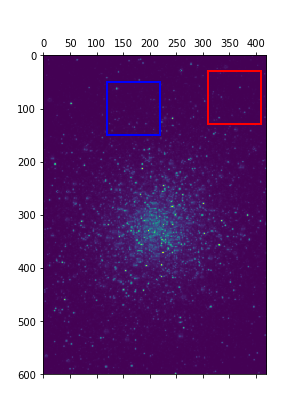
\includegraphics{figures/sdss_m2_image2_marked.png}
    \caption{An image of M2. We trained the wake-sleep algorithm on the red subregion, and evaluated our variational posterior in the blue region. }
    \label{fig:marked_m2}
\end{figure}

\begin{figure}[ht]
\begin{minipage}[b]{0.6\textwidth}
\centering
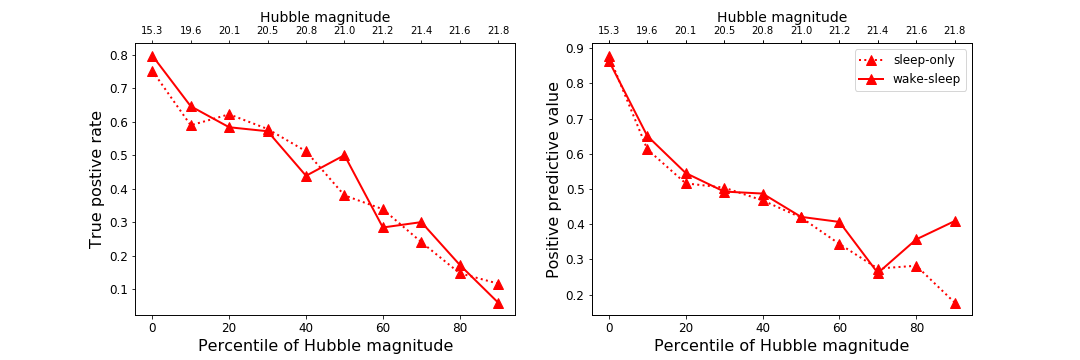
\includegraphics[width = \textwidth]{figures/summary_statistics_m2_alt.png}
\end{minipage}\hfill
\begin{minipage}[b]{0.39\textwidth}
\centering
\begin{tabular}{rrr}
\toprule
     mu &   TPR &   PPV \\
\midrule
 1000.0 &  0.49 &  0.69 \\
 1500.0 &  0.49 &  0.64 \\
 2000.0 &  0.52 &  0.49 \\
\bottomrule
\end{tabular}
\end{minipage}\hfill
\caption{foo}
\end{figure}
